\documentclass[12pt]{article}
%\usepackage[utf8]{inputenc}
\usepackage{geometry}
\usepackage{graphicx} % include images
\usepackage{amsmath, amsthm, amssymb, latexsym} % simbolos de mates y teoremas
\usepackage{hyperref}
\usepackage{caption}
\usepackage{array}
\usepackage{bm} % bold math symbols
\usepackage{relsize} % make math symbols larger/smaller

% Bibliography
\usepackage{biblatex}
\addbibresource{refs.bib}

% Cambiar fuente del documento y de las matemáticas y agregar símbolos
\usepackage[T1]{fontenc}
\usepackage{textcomp}
\usepackage{mathpazo} % paquete de fuente de matemáticas
\usepackage[no-math]{fontspec} % cambiar la fuente del documento
\setmainfont{Roboto-Light}

% Para que los teoremas y definiciones se impriman de la forma:
%   Teorema(Nombre del Teorema)
% Declaramos un nuevo estilo, lo nombramos y le damos el formato
\newtheoremstyle{bfTheoremWithNote} % Nombre del nuevo estilo 
{} % Espacio antes del teorema
{} % Espacio después del teorema
{\itshape} % Tipo de letra para el cuerpo 
{} % Sangría del cuerpo
{\bfseries} % Tipo de letra del titulo
{:} % Puntuacion entre el titulo y el cuerpo del teorema
{\newline} % Espacio despues del titulo del teorema
{\thmname{#1}\thmnumber{}\thmnote{(#3)}}

\newtheoremstyle{bfRemark} % Nombre del nuevo estilo 
{} % Espacio antes del teorema
{} % Espacio despues del teorema
{} % Tipo de letra para el cuerpo 
{} % Sangría del cuerpo
{\bfseries} % Tipo de letra del titulo
{:} % Puntuacion entre el titulo y el cuerpo del teorema
{\newline} % Espacio despues del titulo del teorema
{\thmname{#1 }\thmnumber{}\thmnote{}}
    
\theoremstyle{bfTheoremWithNote}
\newtheorem{lemma}{Lema}
\newtheorem{definition}{Definición}
\newtheorem{theorem}{Teorema}
\newtheorem{corollary}{Corolario}
\newtheorem{proposition}{Proposición}

\theoremstyle{bfRemark}
\newtheorem{remark}{Nota}

% Defino comandos útiles para mí

        % Simbolos especiales
        \newcommand{\transpose}{{\scalebox{0.65}{$\top$}}}
        \newcommand{\inverse}{{\scalebox{0.65}{$-1$}}}
        \newcommand{\gen}[1]{\mathnormal{gen}\{#1\}}
        \newcommand{\eulerconstant}{\scalebox{1.2}{e}}
    
        % Conjuntos de Numeros
        \newcommand{\feal}{\mathbb{F}}
        \newcommand{\Real}{\mathbb{R}}
        \newcommand{\Natural}{\mathbb{N}}
        \newcommand{\Whole}{\mathbb{Z}}

\title{El problema del agente viajero}
\author{Mauricio Trejo \and Alejandra \and Andrés}
\date{7 de diciembre de 2019}

\begin{document}

\maketitle

\section{Planteamiento del problema}

Supongamos que tenemos $k$ ciudades conectadas por rutas bidireccionales.

Un agente de ventas que reside en la ciudad 1 debe viajar a cada una de las ciudades al menos una vez y después regresar a su hogar. 

El problema del agente viajero consiste en encontrar el trayecto que atraviese todas las ciudades y cuya distancia sea mínima.

    \subsection{Planteamiento gráfico}

        Sea $\mathcal{G}$ la gráfica que representa este problema, entonces
        \begin{enumerate}
            \item el conjunto de los nodos de $\mathcal{G}$ queda dado por $\mathcal{N}_\mathcal{G} = \{n_1, n_2, \dots, n_k\}$ donde cada nodo representa una ciudad. 
            \item el conjunto de los arcos de $\mathcal{G}$ queda dado por $\mathcal{A}_\mathcal{G} = \{ a_{ij} \; | \; i \neq j, \; i,j = 1, 2, \dots, k \}$ donde cada elemento $a_{ij}$ representa la ruta entre la ciudad $i$ y la ciudad $j$.
            \item el conjunto de distancias $\mathcal{D}$ queda dado por $\mathcal{D} = \{ d_{ij} \; | \; i \neq j, \; i,j = 1, 2, \dots, k \}$ donde $d_{ij}$ representa la distancia del arco $a_{ij}$. 
        \end{enumerate}

    \subsection{Planteamiento algebráico}

        Sea $x_{ij}$ para $i,j = 1, 2, \dots, k$, $i \neq j$ tal que
        \begin{equation*}
            x_{ij} = 
            \begin{cases}
                1 &\text{si el arco $a_{ij}$ está en la ruta óptima} \\
                0 &\text{e.o.c} 
            \end{cases}
        \end{equation*}
        
        El problema del agente viajero se puede plantear como un PLE de la manera siguiente:
        \begin{equation}
            \begin{aligned}
                &\text{minimizar}   &&\sum_{i = 1}^k \sum_{i \neq j = 1}^k d_{ij} x_{ij}\\
                &\text{sujeto a}    &&\sum_{i = 1}^k \sum_{i \neq j = 1}^k x_{ij} \geq k\\
                &                   &&d_{ij} \in \Natural, x_{ij} \in \{0, 1\} \quad \forall i,j = 1, 2, \dots, k, i \neq j
            \end{aligned}
        \end{equation}

\section{Algoritmos genéticos}

    La mayoría de los algoritmos de optimización y búsqueda clásicos utilizan un procedimiento determinístico para alcanzar una solución óptima: comienzan desde un punto cualquiera y determinan la dirección de búsqueda mediante una regla predeterminada \cite{IMD2004}. 
        
    La naturaleza determinística de los métodos tradicionales tiene las siguientes desventajas:
    \begin{enumerate}
        \item La convergencia a una solución optimal depende de la solución inicial de la que se parte.
        \item Pueden quedar atrapados en óptimos locales.
        \item No son eficientes en el proceso de solución de problemas con un espacio de búsqueda discreto.
    \end{enumerate}
    Los dos primeros problemas se pueden resolver mediante la aleatoriedad, pero el último no.

    La \textit{computación evolutiva} se refiere a un conjunto de algoritmos estocásticos de búsqueda que se basan de una forma u otra en la idea del proceso de la evolución de Darwin. Su mayor atributo es que no sufren de los males que aquejan a los algoritmos clásicos.
    
    El funcionamiento de los algoritmos evolutivos se puede resumir de manera general en cuatro pasos \cite{IMD2004}:
    \begin{enumerate}
        \item Se mantiene una población de posibles soluciones para el problema.
        \item Se modifican las soluciones almacenadas y se descartan algunas de acuerdo con una medida de adaptación al entorno.
        \item El proceso de modificación y selección obliga a la población a evolucionar a través de las mejores regiones del espacio de búsqueda.
        \item Las modificaciones hechas a la población permiten mezclar información de los padres que se transmite a los descendientes (\textit{cruce}) o introducir innovación dentro de la población (\textit{mutaciones}).
    \end{enumerate}

    Los algoritmos genéticos se distinguen de los demás algoritmos evolutivos por tres razones: su esquema binario, el método de selección que utilizan y el uso del cruce de información para producir variaciones en la población \cite{IMD2004}. 

    \textbf{Algoritmo genetico (reescribir como lista)}: el sistema parte de una población inicial de individuos que codifican, mediante alguna representación genética, soluciones candidatas al problema propuesto. Esta población de individuos (a los que se denomina cromosomas) evoluciona en el tiempo a través de un proceso de competición y variación controlada. Cada cromosoma de la población tiene asociada una medida de adaptación para determinar qué cromosomas serán seleccionados para formar parte de la nueva población en el proceso de competición. La nueva población se creará utilizando operadores genéticos de cruce y mutación. Este ciclo evolutivo continúa hasta que se verifique una determinada condición de parada: que se hayan realizado un determinado número máximo de evaluaciones de individuos, que la población haya evolucionado durante un número máximo de generaciones, que se haya alcanzado una solución con un determinado valor de la función de adaptación (o de parte de ella), que se estacione la población por no generarse individuos nuevos durante un determinado número de generaciones, etc. 

    \begin{figure}[h]
        \centering
        \label{fig:flowchart-gen-algorithm}
        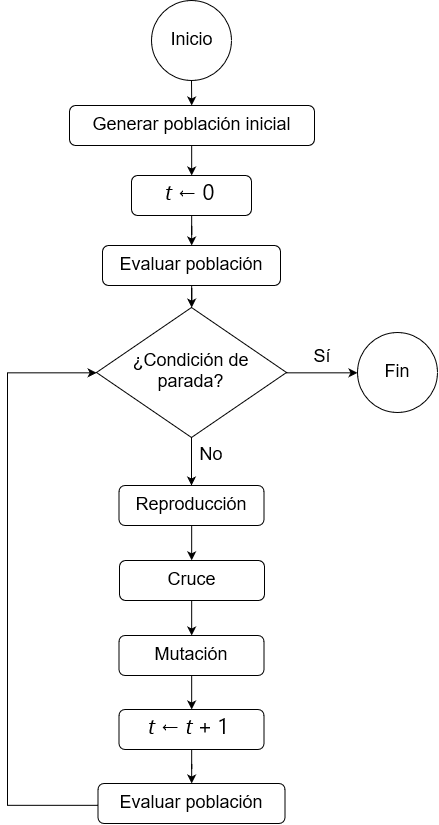
\includegraphics[width = 0.5\textwidth]{Images/flowchart-gen-algorithm.png}
        \caption{Diagrama de flujo de un Algoritmo Genético básico}
    \end{figure}

    \section{Explicación del código}



\end{document}